\section{Parallel algorithms}
\label{sec:parallel}

In this section, we present a parallelization of the color coding approach using
MapReduce framework, we will first describe \sahad{}
\cite{zhao2012sahad}, followed by  \ensahad{} and  \harpsahad{} respectively.

\subsection{\sahad{}}
\label{sec:sahad-implementation}

\sahad{} takes a sequence of templates $\mathcal{T}=\{T_0,...,T\}$ as
input. Here $\mathcal{T}$ represents a set of templates generated by
partitioning $T$ using Algorithm~\ref{alg:partition}. Then it performs MapReduce
variation of Algorithm~\ref{alg:sequential} to compute the number of embeddings
of $T$. 

As shown in Equation~\ref{eq:color-coding-dp}, the counts of all colorful embeddings
isomorphic to $T$ rooted from a single node $v$ is computed by aggregating the
same measurement of $T'$ and $T''$, i.e., the two sub-templates, with $T'$
rooted from $v$ and $T''$ rooted from $\forall u \in N(v)$. We can parallelize
color-coding algorithm by distributing the computation among multiple machines,
and sending data related with $v$ and $N(v)$ to a computation unit for the
aggregation. In our MapReduce algorithm, we manage this by assigning $v$ as the
key for both the counts of $T'$ rooted at $v$ and the counts of $T''$ rooted
at $v$'s neighbors, such that all data required for computing counts for
$T$ rooted at $v$ has the same key and will be handled by a single reduce
function.

%We hereby define the notation $X_{T, v}$ since we will be using it in the
%algorithms presented in this paper. 
Let $X_{T, v}$ be a sequence of color-count
pairs $(S_0=\{s_1^0, s_2^0, ..., s_k^0\}, c_0), (S_1=\{s_1^1, s_2^1, ...,
s_k^1\}, c_1),...$, where $S_i$ represent a color set containing $k$ colors, and
$c_i$ is the counts of the subgraphs isomorphic to $T$ and rooted at $v$ that
are colored by $S_i$. Here $k = |V(T)|$, and each subgraph is a colorful match.

There are 3 types of Hadoop jobs in \sahad{}, which are 1) colorer
(Algorithm~\ref{alg:colorer-mapper}) that performs line 4 of Algorithm
~\ref{alg:sequential}; 2) counter (Algorithm~\ref{alg:counter-mapper},
~\ref{alg:counter-reducer}) which performs line 6 of Algorithm
~\ref{alg:sequential} and 3) finalizer (Algorithm~\ref{alg:sum-mapper},
~\ref{alg:sum-reducer}) that performs line 7 of Algorithm~\ref{alg:sequential}. 

The first step is to random color network $G$ with $k$ colors. The map function 
is described in Algorithm~\ref{alg:colorer-mapper}:

\begin{algorithm}[ht]
  \caption{\emph{mapper($v, N(v)$)}}
  \label{alg:colorer-mapper}
  \begin{algorithmic}[1]
    \STATE Pick $s_i \in \{s_1,\ldots,s_k\}$ uniformly at random\\
	\STATE color $v$ with $s_i$
	\STATE Let $T_0$ be the single node template
	\STATE Let $c(v, T_0, \{s_i\})=1$ since $v$ is the only colorful matching\\
    \STATE $X_{T_0, v} \leftarrow \{(\{s_i\}, 1)\}$ \\
    \STATE Collect($\underline{key \leftarrow v}, \underline{value \leftarrow X_{T_0, v}, N(v)}$)
  \end{algorithmic}
\end{algorithm}

Here ``Collect'' is a standard MapReduce operation that will emit the key-value
pairs to global space for further process such as shuffling, sorting or I/O.
$N(v)$ represents the neighbors of $v$. Note that template $T_0$ is a single
node, therefore $X_{T_0, v}$ contains only a single color-count pair $({s_v}, 1)$

According to Equation~\ref{eq:color-coding-dp}, to compute $X_{T_i, v}$, we need $X_{T'_i, v}$ for
sub-template $T'_i$ and $X_{T''_i, u}$ for all $u \in N(v)$ for sub-template
$T''_i$. We use a mapper and a reducer function to implement this as shown in
Algorithm~\ref{alg:counter-mapper} and \ref{alg:counter-reducer}, respectively.

\begin{algorithm}[ht]
  \caption{\emph{mapper($v, X_{t, v}, N(v)$)}}
  \label{alg:counter-mapper}
  \begin{algorithmic}[1]
    \IF{$t$ is $T'_i$}
      \STATE Collect($\underline{key \leftarrow v}, \underline{value \leftarrow X_{t, v}, flag'}$)
    \ELSE
      \FOR{$u \in N(v)$}
        \STATE Collect($\underline{key \leftarrow u}, \underline{value \leftarrow X_{t, v}, flag''}$)
      \ENDFOR
    \ENDIF
  \end{algorithmic}
\end{algorithm}

Note that in Algorithm~\ref{alg:counter-mapper}, the second \textit{Collect} emits
$X_{T''_i, v}$ to all its neighbors. Therefore, as shown in Algorithm
~\ref{alg:counter-reducer}, $X_{T'_i, v}$ and $X_{T''_i, u}$ from all $u \in
N(v)$ are handled by the same reducer, which is sufficient for computing Eq.
~\ref{eq:color-coding-dp}. Also note that for a given node
$v$, the number of entries with $flag'$ is 1, and the number of entries with
$flag''$ equals $|N(v)|$.


\begin{algorithm}[ht]
  \caption{\emph{reducer($v, {(X, flag), (X, flag), ...}$)}}
  \label{alg:counter-reducer}
  \begin{algorithmic}[1]
    \STATE pick $X_1$ where $flag = flag'$
      \FOR {all colorset $S'_i$ from $X_1$}
 \FOR {each $X$ other than $X_1$} 
   \FOR {all colorset $S''_i$ from $X$}
     \IF {$S'_i \cap S''_i = \emptyset$}
              \STATE $c(v, T_i, S'_i \cup S''_i) += 1$
            \ENDIF
          \ENDFOR
        \ENDFOR
      \ENDFOR 
    \STATE Collect($\underline{key \leftarrow v}, \underline{value \leftarrow X_{T_i, v}, N(v)}$)
  \end{algorithmic}
\end{algorithm}

The last step is to compute the total count described in Eq.
~\ref{eq:color-coding-sum}, and is shown in Algorithm \ref{alg:sum-mapper} and
~\ref{alg:sum-reducer}.

\begin{algorithm}[ht]
  \caption{\emph{mapper($v, X_{T, v}, N(v)$)}}
  \label{alg:sum-mapper}
  \begin{algorithmic}[1]
      \STATE Collect($\underline{key \leftarrow ``sum''}, \underline{value \leftarrow X_{T, v}}$)
  \end{algorithmic}
\end{algorithm}

\begin{algorithm}[ht]
  \caption{\emph{reducer($``sum'', {X_{T, v_1}, {X_{T, v_2},...}}$)}}
  \label{alg:sum-reducer}
  \begin{algorithmic}[1]
    \STATE $Y = \frac{m^m}{m!} \cdot \frac{1}{q}\sum_{\forall v \in V_G}X$
    \STATE Collect($\underline{key \leftarrow ``sum''}, \underline{value \leftarrow X_{T, v}}$)
  \end{algorithmic}
\end{algorithm}

Note that in Algorithm~\ref{alg:sum-mapper}, $X_{T,v}$ only contains one
element, which is the count corresponding to the entire color set. Then in the
reducer shown in Algorithm~\ref{alg:sum-reducer}, all the counts are added
together and properly factorized, to obtain the final count. For a
comprehensive description of the MapReduce version of color coding, please
refer to~\cite{zhao2012sahad}.

\subsection{\ensahad}
\label{sec:ensahad}

For general MapReduce problem, the set of keys that is processed in Mapper and
Reducer varies among different jobs. Therefore, MapReduce uses external
shuffling and sorting in-between Mappers and Reducers to deploy the keys to
computing nodes. 

In our algorithm, however, the dynamic programming aggregates counts based on
the root node of the subtree, and therefore the key is the node index $v$.  In
\ensahad{}, we use this pre-knowledge to predefine a reducer that is
corresponding to a set of nodes. We also assign the predefined reducers to
computing nodes prior to the beginning of the dynamic programming. Therefore, a
data entry with key $v$ will be directly sent to the corresponding computing
node and processed by designated Reducer. Using this mechanism, we can reduce
the cost of shuffling and sorting in intermediate stage of Hadoop jobs.

\iffalse
In addition, the network communication cost among computing nodes is also a
bottleneck in most of the parallellization frameworks. With the predefined
reducers, the communication cost is $O(E_{out})$. Here $E_{out}$ represents the
number of edges among partitions. To study the performance variations regarding
$E_{out}$, we explore different partitioning schemes for distributing graph data
to computing nodes.  Some partitioning schemes may introduce lower number of
inter-partition edges $E_{out}$, but higher number of intra-partition edges.
Here we investigate two partitioning schemes: the random partitioning and
min-cut partitioning.

We use~\cite{Web:metis} to perform minimum cut partitioning with the following
two constraints: a) divide the network into partitions with roughly the same
size, b) minimize the number of inter-partition edges. The purpose is to
maintain load balancing among computing nodes, and reduce the communication cost
$O(E_{out})$ by minimizing the number of inter-partition edges.

\fi


\subsection{\harpsahad{}}
\label{sec:harp-implementation}

\begin{figure}[htbp]
\centerline{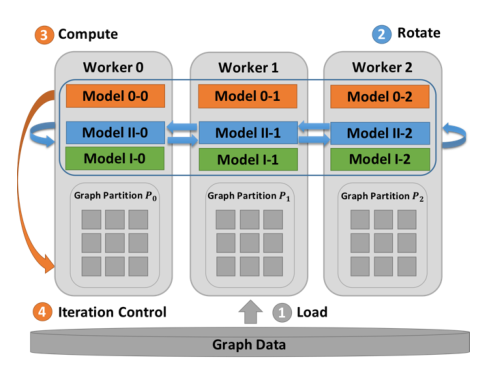
\includegraphics[width=0.36\textwidth]{plots/harp-imp.eps}}
\caption{Here shows one iteration of the Harp implementation. $P_0$ through
$P_2$ are parts of a partition of graph $G$}
\label{fig:harp-imp}
\end{figure}


Figure~\ref{fig:harp-imp} illustrates \harpsahad{} for one iteration
that counts the embeddings of the template $T$ based on the embeddings of
sub-template $T'$ and $T''$.  Graph data is partitioned and stored separately on
each worker node in the form of adjacency list. Partitioned graph data is loaded
and cached in memory. The model represents a data structure including a
color-count pairs for each vertex in graph. Since it follows the dynamic
programming scheme, computation runs with static partitioned graph and multiple
template models. Model updates are achieved with Model I (embeddings of
sub-template $T'$) and model II (embeddings of sub-template $T''$) generating
embeddings of template $T$ on model 0. Note that model I and model II are
partitioned and stored separately on the cluster. The model distribution
approach with rotation can effectively reduce memory usage per node, thereby
addressing the issue when graph template models become too large to fit into
memory.


Note that only model II rotates among the worker nodes. As such, it takes three
rounds to complete updating model 0 in Figure~\ref{fig:harp-imp}. In the first round, 
it joins model I-0 and model II-0 to generate new values for model 0-0. Then all
parts of model II
rotate so that model II-2 is accessible on worker 0. In the second round, it
joins model I-0 and model II-2 and updates model 0-0. Again, it rotates so that
model II-1 is now accessible to worker 0. It then joins model I-0 with model II-1
and updates model 0-0. After this rotation, worker 0 is given access to all
parts of model II and complete updating model 0 in one iteration. Worker 1
and worker 2 run in the same way in parallel. At each iteration, the embeddings 
of sub-template $T'$ and $T''$ are used for updating the embeddings of the parent 
template $T$. Harp model rotation achieves scaling for fine-grained graph
model synchronization with in-memory collective communication.

